%%%%%%%%%%%%%%%%%%%%%%%%%%%%%%%%%%%%%%%%%%%%%%%%%%%%%%%%%%%%%%%%%%%%%%%%%%%%%%
%
% Topico     : Estilo de Informes - DMCC  
% Autor      : Ruben Carvajal Schiaffino
% Santiago de Chile, 13/9/2016
%
%%%%%%%%%%%%%%%%%%%%%%%%%%%%%%%%%%%%%%%%%%%%%%%%%%%%%%%%%%%%%%%%%%%%%%%%%%%%%%
% 
%
\documentclass{report}
%
%
%
\usepackage[spanish]{babel}
\usepackage{epsfig}
%
\usepackage{pdfpages}
\usepackage{float}
\usepackage{array}
\usepackage[utf8]{inputenc}
\usepackage[toc,header,title]{appendix}
\usepackage{graphicx}
\usepackage{booktabs}
\usepackage{algorithm}
\usepackage{algpseudocode}
\graphicspath{{./images/}}
%
\renewcommand*\thesection{\arabic{section}}
\newcommand \tab{\hspace*{25 pt}}
\newcommand \minitab{\hspace*{15 pt}}
\usepackage[pagestyles]{titlesec}
\titleformat{\chapter}[display]{\normalfont\bfseries}{}{0pt}{\Huge}
\newpagestyle{mystyle}
{\sethead[\thepage][][\chaptertitle]{}{}{\thepage}}
\pagestyle{mystyle}
%
\begin{document}
\begin{titlepage}
\begin{center}
%\psfig{figure=L-USACH-16.png,height=3cm,,}
\end{center}
\begin{center}
{\bf Departamento de Matem\'atica y Ciencia de la Computaci\'on}
\end{center}
\vspace{3cm}
\begin{center}
%%%%%%%%%%%%%%%%%%%%%%%%%%%%%%%%%%%%%%%%%%%%%%%%%%%%%%%%%%%%%%%%
%
% MODIFICAR. Despues del tag \bf se coloca el titulo del trabajo
%
{\Large \bf Primer examen}
%
%%%%%%%%%%%%%%%%%%%%%%%%%%%%%%%%%%%%%%%%%%%%%%%%%%%%%%%%%%%%%%%%
%
\end{center}
\begin{center}
%
%%%%%%%%%%%%%%%%%%%%%%%%%%%%%%%%%%%%%%%%%%%%%%%%%%%%%%%%%%%%%%%%
%
% MODIFICAR. Despues del tag \bf se coloca el semestre y año
%
{\large \bf Segundo Semestre 2018}
%
%%%%%%%%%%%%%%%%%%%%%%%%%%%%%%%%%%%%%%%%%%%%%%%%%%%%%%%%%%%%%%%%
%
\end{center}
\vspace{5cm}
\begin{tabular}{c l c}
%
%%%%%%%%%%%%%%%%%%%%%%%%%%%%%%%%%%%%%%%%%%%%%%%%%%%%%%%%%%%%%%%%
%
% MODIFICAR. En el primer campo colocar el nombre de la asignatura y su codigo
%            En el segundo campo colocar el nombre del autor
%
Algoritmos Distribuidos 26106 & ~~~~~~~~~~~~~~~~~ & Rafael A. Castillo L\'opez \\
%
%%%%%%%%%%%%%%%%%%%%%%%%%%%%%%%%%%%%%%%%%%%%%%%%%%%%%%%%%%%%%%%
%
% MODIFICAR. En el primer campo colocar el nombre de la carrera
%            En el segundo campo color direccion electronica
%
Licenciatura en Ciencia de la Computaci\'on & ~~ & rafael@trfs.me
%
%%%%%%%%%%%%%%%%%%%%%%%%%%%%%%%%%%%%%%%%%%%%%%%%%%%%%%%%%%%%%%%
%
\end{tabular}
\end{titlepage}

\chapter{Problema 1}

\textbf{Enunciado} Haz un estudio del comportamiento del algoritmo que determina
la distancia de estrellas a partir de una matriz de intensidad de luz. La
implementaci\'on vista en clase recorre la matriz por filas. Construya una
implementaci\'on que la recorra por columnas y haga una comparaci\'on entre
las secuenciales y las paralelas. Recuerde que en clase se vieron dos metricas
para medir el rendimiento.

\section{Algoritmo}

El algoritmo por filas es el mismo visto en clase, y solo se necesitan
realizar cambios triviales para obtener la versión por columnas.

\section{Analis\'is de complejidad}

Ambos algoritmos secuenciales tienen complejidad lineal con respecto al numero
de elementos de la matriz de entrada. Es decir que para una matr\'iz de tamaño
$N \times M$. El algoritmo ser\'a $\mathcal{O}(MN)$.

\section{Experimentos}

Todos los experimentos se corrieron en un servidor con las especificaciones presentadas en la tabla
~\ref{table:testspecs}.

\begin{table}[H]
  \begin{tabular}{ >{\bf}l l }
  Procesador & Dos Intel Xeon Gold 6126 CPU @ 2.60GHz \\
  Numero de nucleos & 12 por procesador, 24 en total (48 hilos con Hyper Threading) \\
  Memoria ram & 128 GiB \\
  Sistema operativo & Ubuntu 16.04 x86-64 \\
  Memoria secundaria & SSD Samsung MZ7KM240HMHQ0D3 de 240 GiB\\
  Nucleo & Linux 4.4.0-138 \\
  Compilador & Clang 6.0
\end{tabular}
\caption{Especificaciónes del entorno de prueba}
\label{table:testspecs}
\end{table}

Se corr\'io cada algoritmo con matrices cuadradas de $N \times N$  para 
$N = 500, 1000, 1500 \ldots 9500, 10000 $. Como escalamos ambas
dimensiones de la matr\'iz al mismo tiempo y en las graficas de
rendimiento usaremos solo $N$ como eje $x$, para efectos de este experimento
el algoritmo se comportar\'a con complejidad $\mathcal{O}(N^2)$.

Cada punto de prueba se ejecut\'o con ambos algoritmos secuenciales, y
con ambos algoritmos paralelos con 3, 6, 12, 24, 48 y 96 hebras (empezamos de
3 ya que nuestro procesador tiene un n\'umero de nucleos multiplo de 3). Se
realizaron ademas 40 repeticiones del experimento y se tomo el valor mediano
para presentar resultados. Las tablas con los resultados resumidos se encuentran
en el ap\'endice \ref{appendix:starresults}.

En la figura \ref{fig:starperf} se muestran los tiempos de ejecución de ambos
algoritmos. Observamos que aunque teóricamente ambos algoritmos tengan
comportamientos asimptoticos exactamente iguales, ¡el algoritmo por columnas toma
casi el doble de tiempo que el algoritmo por filas! Esto probablemente se debe a
que la baja localidad de datos en el caso por columnas lleva a muchos fallos de
cache. Tambien se vé que los algoritmos paralelos ofrecen una mejora dramatica
sobre los secuenciales, aunque su comportamiento no sea tan estable.

\begin{figure}[h]
    \centering
  \caption{Izquierda: rendimiento de los algoritmos por fila. Derecha: rendimiento
           de los algoritmos por columna.}
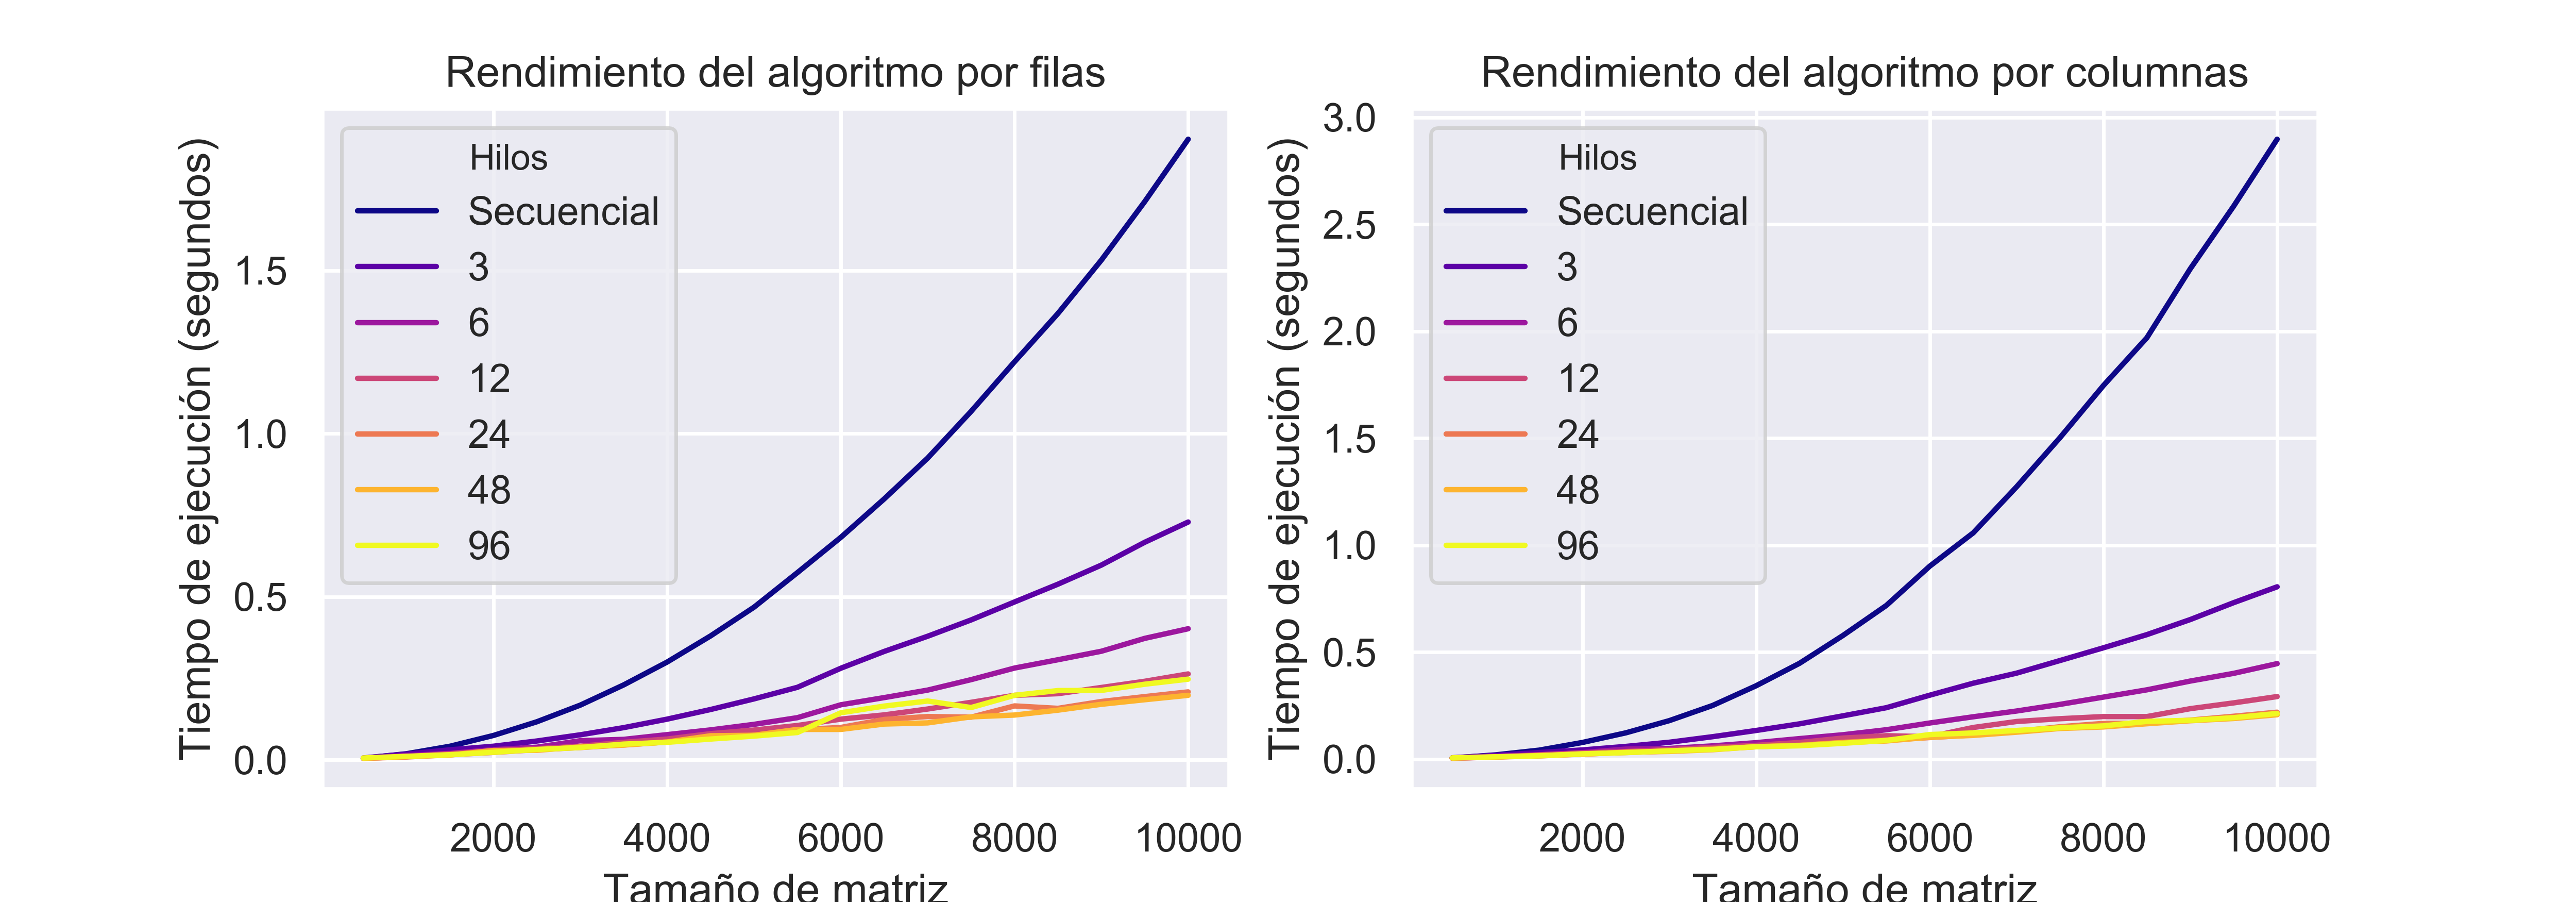
\includegraphics[width=\textwidth]{stars_perf}
\label{fig:starperf}
\end{figure}

La figura \ref{fig:starperfbar} nos muestra el rendimiento para el caso especifico
de una matríz de $10000 \times 10000$. Aqui se aprecia mejor como mejora el rendimiento con
mas hilos. Curiosamente podemos ver en el algoritmo por filas que el rendimiento
con 96 hilos es peor que el rendimiento con 48. 48 hilos es el maximo que el
procesador usado en las pruebas puede correr en paralelo (contando los nucleos
virtuales o HyperThreads). Esto no se presenta en la versión por columnas.
Hipotetizo que la razón de esto es que aunque el mas rápido algoritmo por filas
llegue a un cuello de botella ocasionado por el cambio de contexto entre hilos,
el algoritmo por columnas aún es limitado por su mas lento acceso a memoria.

\begin{figure}[H]
    \centering
  \caption{Rendimiento para una matriz de $10000 \times 10000$}
  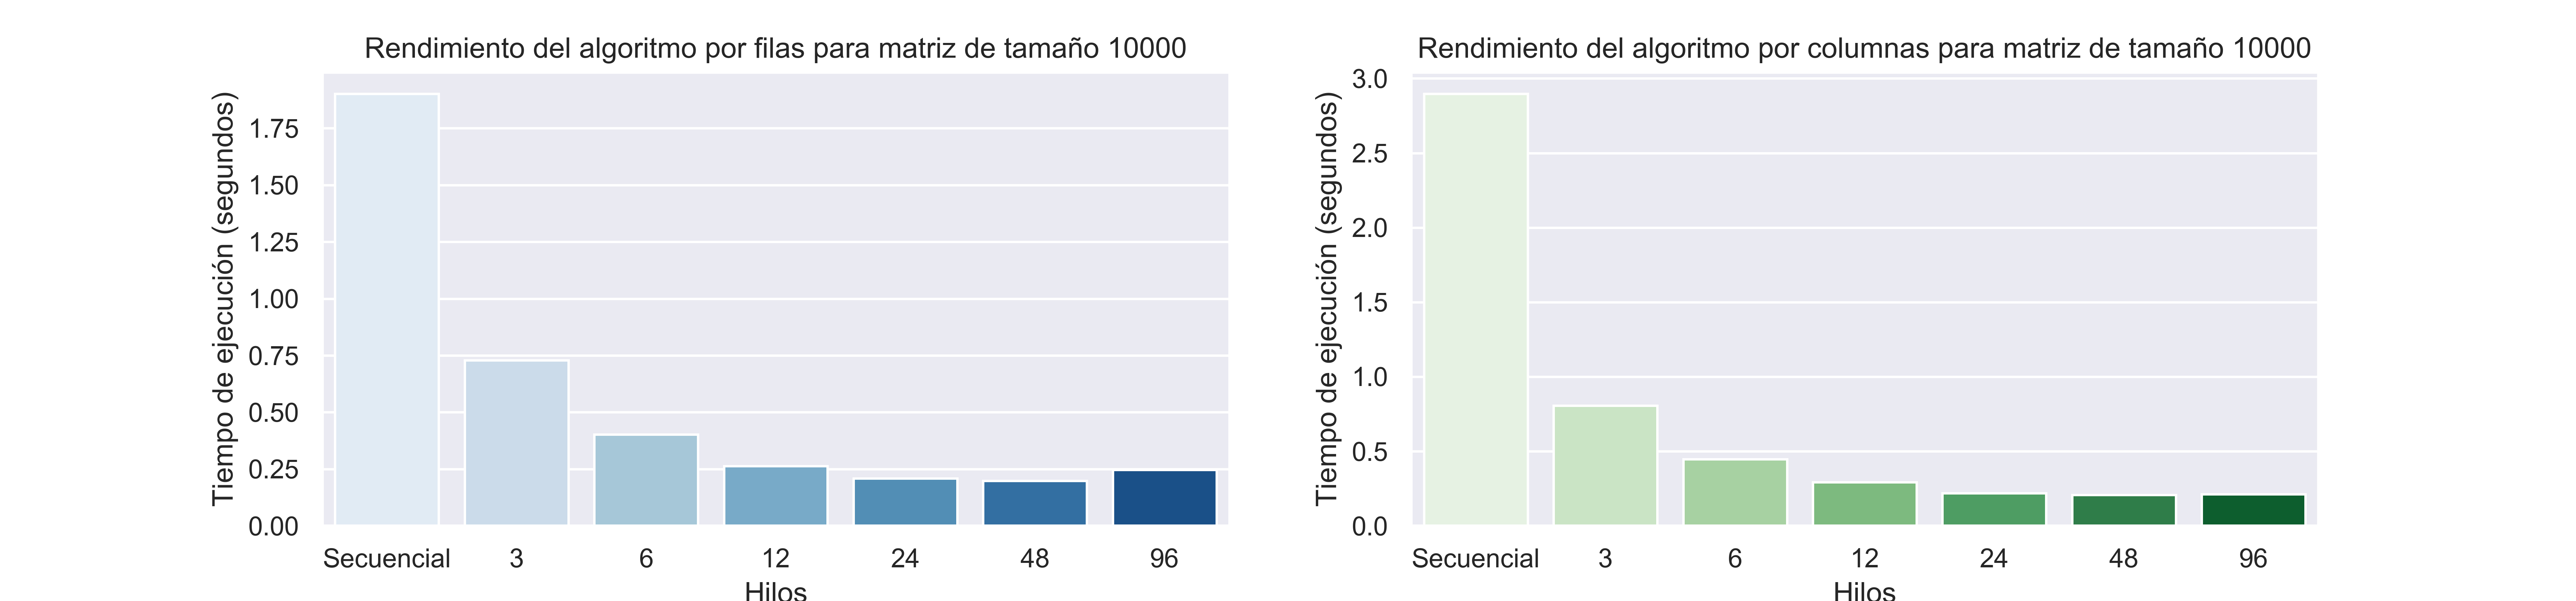
\includegraphics[width=\textwidth]{stars_perf_bar}
\label{fig:starperfbar}
\end{figure}

En el mapa de calor de la figura \ref{fig:staraccel} podemos ver la aceleración de
los algoritmos probados. Podemos ver la tendencia general de que la aceleración
crezca con el numero de hilos y el tamaño del problema, con la excepción previamente
mencionada del algoritmo por filas usando 96 hilos.

\begin{figure}[H]
    \centering
  \caption{Mapa de calor de aceleración}
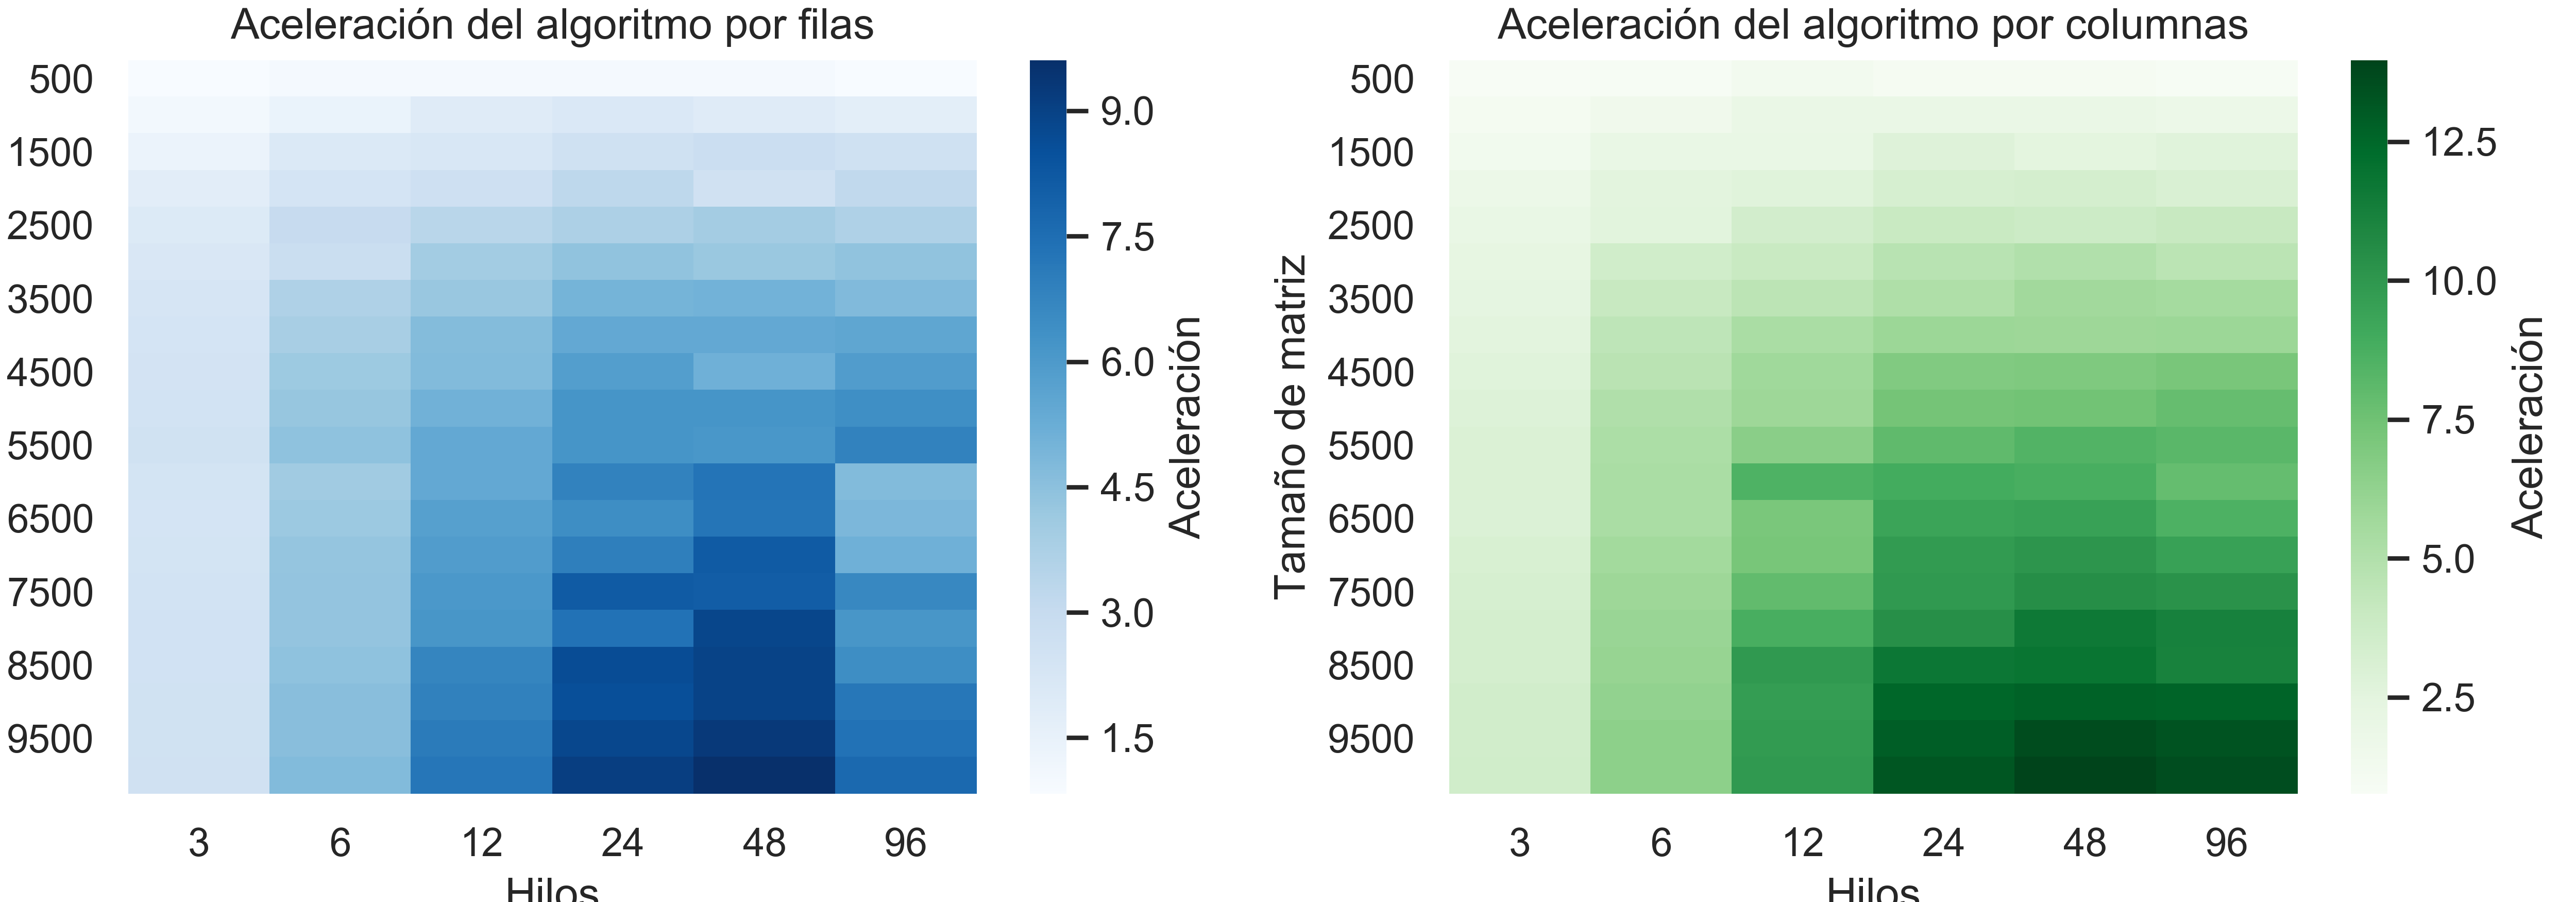
\includegraphics[width=\textwidth]{stars_accel}
\label{fig:staraccel}
\end{figure}

De nuevo acercandonos a nuestro caso extremo de la mátriz de $10000 \times 10000$ en
la figura \ref{fig:staraccelbar}, observamos que en ambos casos nuestra aceleración
crece hasta cierto punto mientras mas hilos agreguemos, aunque nuestra delta de
aceleración baje entre mas hilos empleemos. Tambien vemos el comportamiento con 96
hilos en ambos casos: en el algoritmo por columnas, no vemos mejora al agregar estos
hilos, mientras que en el algoritmo por filas, perdemos tiempo, como se habia
mencionado antes.

\begin{figure}[H]
    \centering
  \caption{Aceleración para mátriz de $10000 \times 10000$}
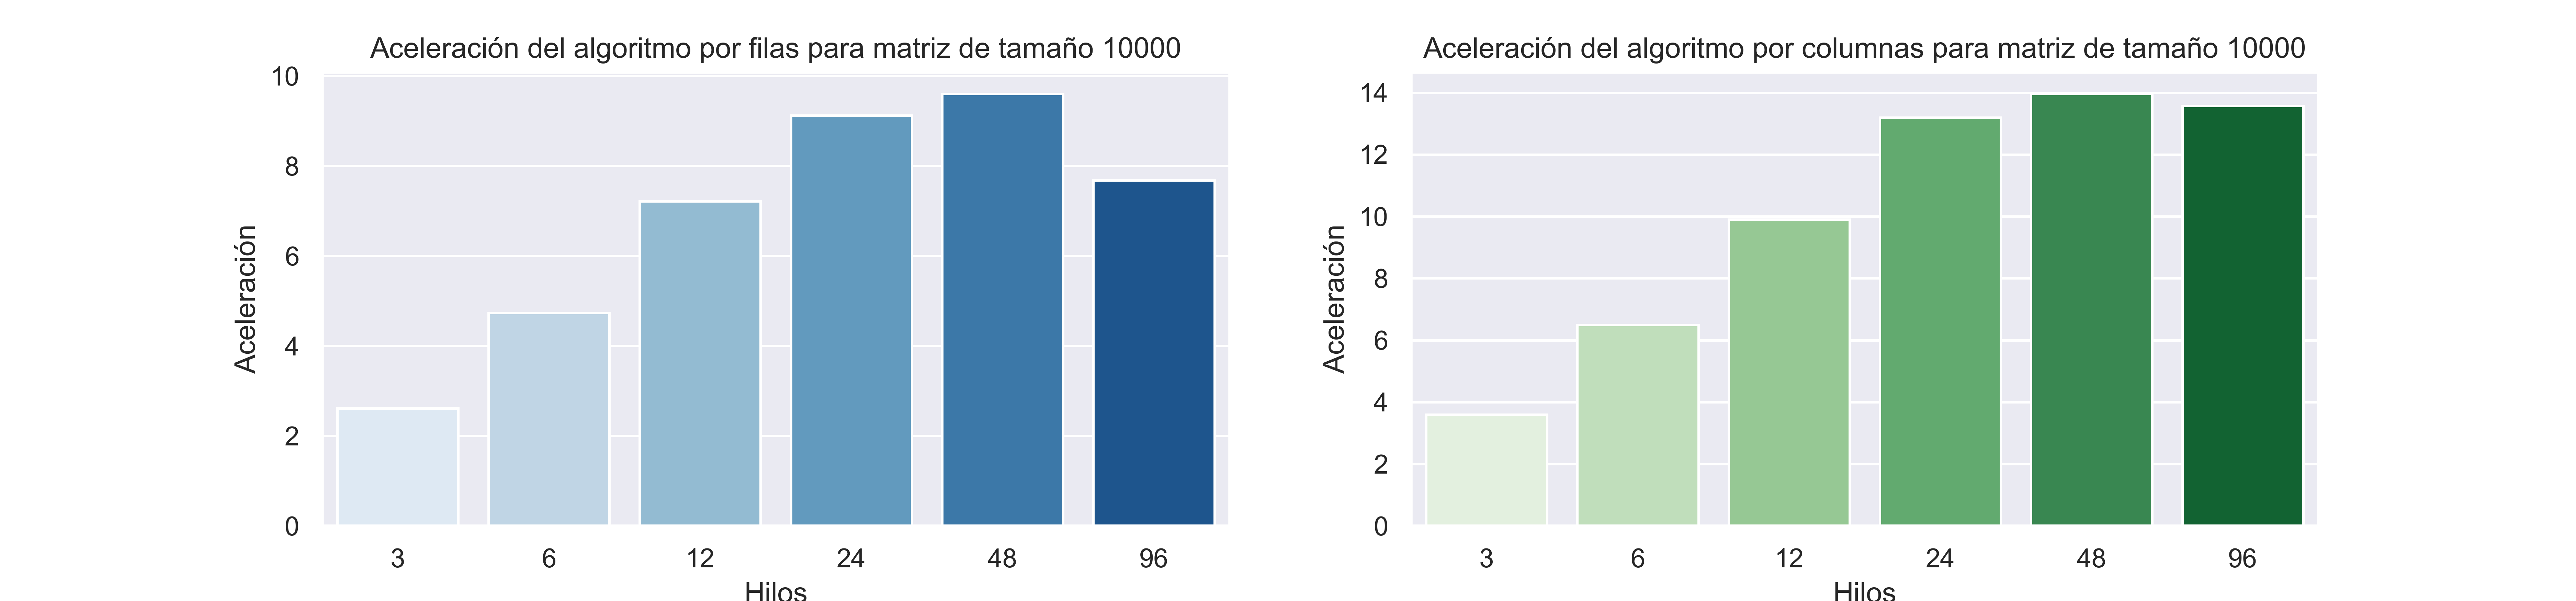
\includegraphics[width=\textwidth]{stars_accel_bar}
\label{fig:staraccelbar}
\end{figure}

En el caso de la eficiencia, vemos una historia muy parecida para ambos algoritmos.
Aunque el tiempo que toman menos tiempo real, la eficiencia del uso de recursos
en realidad baja dramaticamente aumentando el número de hilos. La figura
\ref{fig:stareff} muestra este comportamiento.

\begin{figure}[H]
    \centering
  \caption{Mapa de calor de eficiencia}
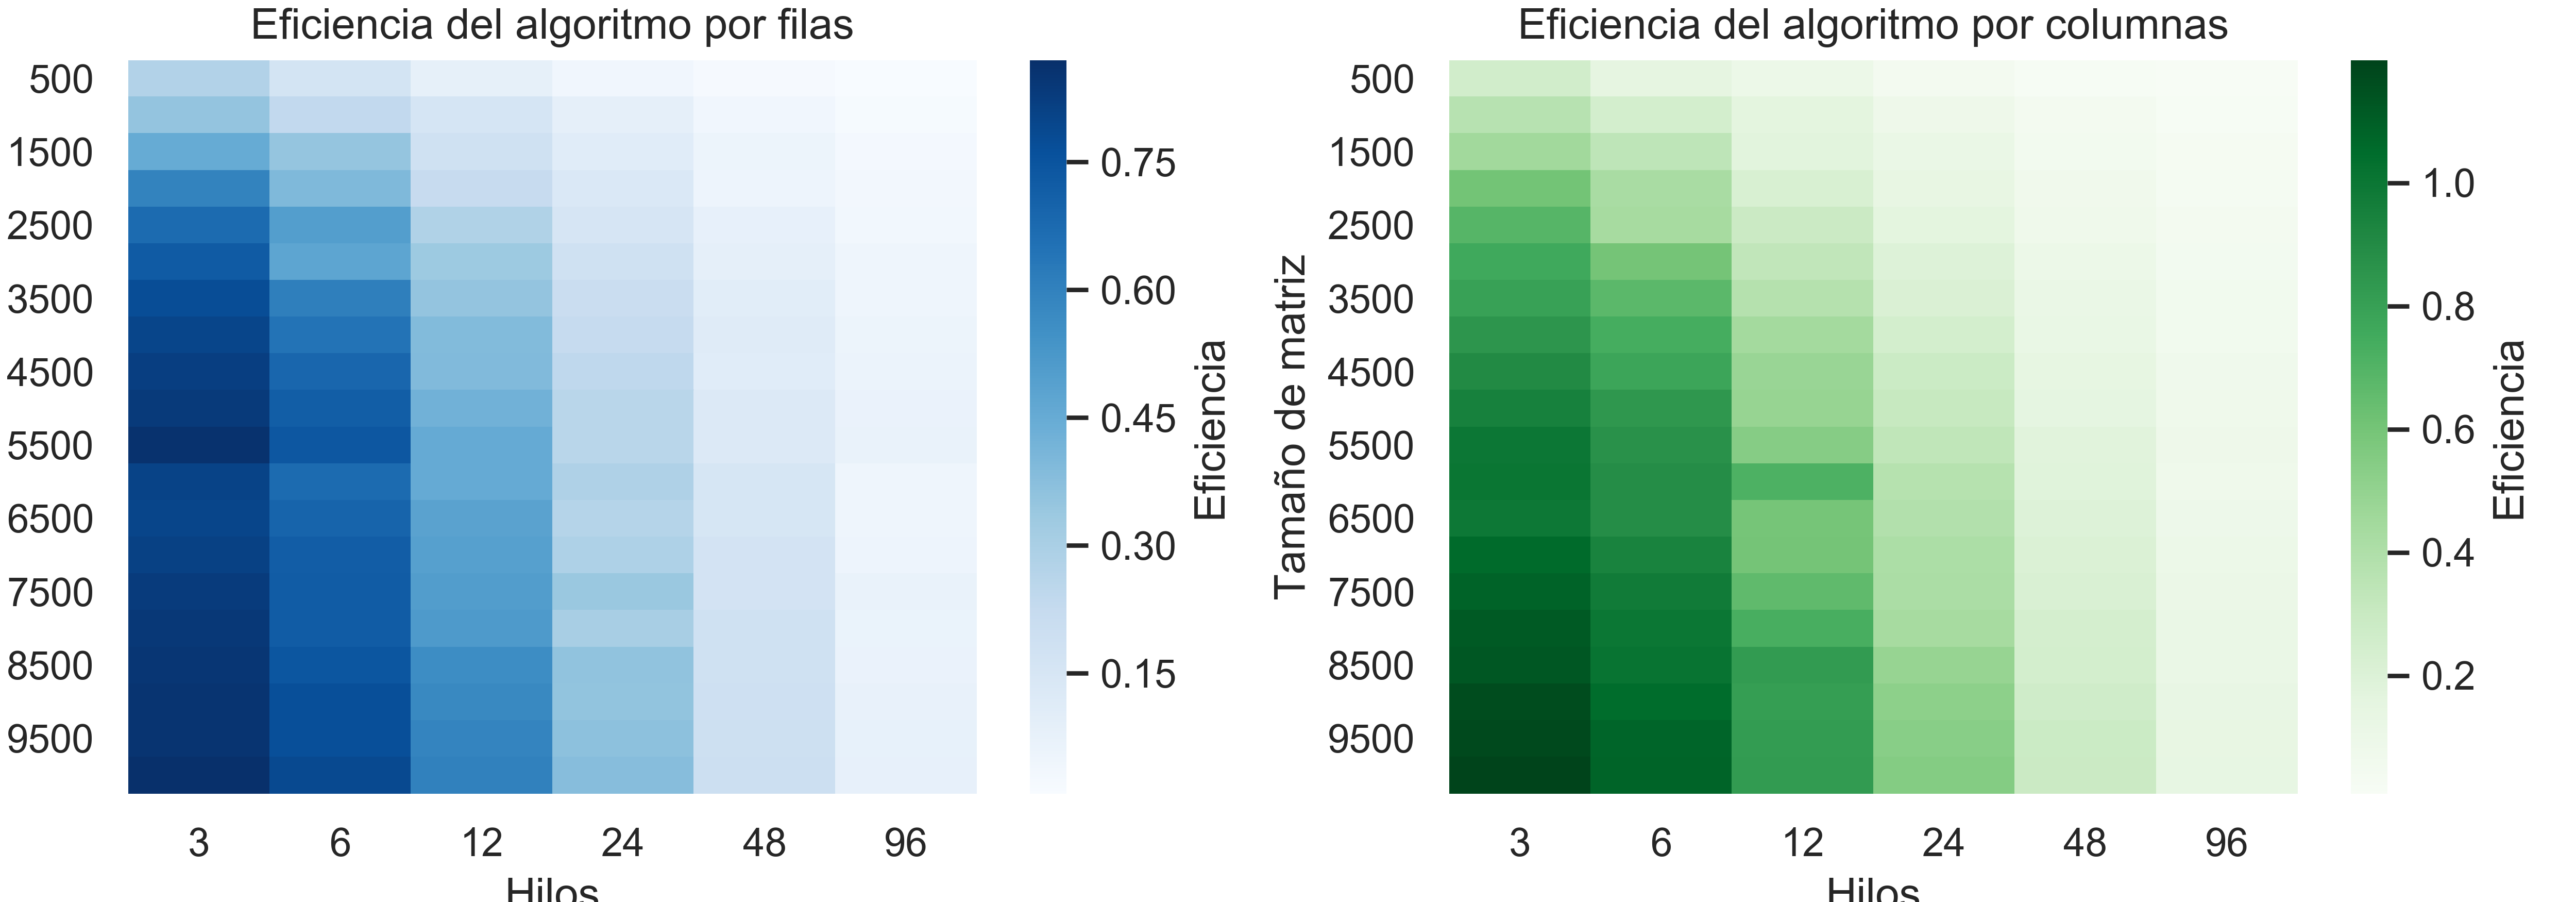
\includegraphics[width=\textwidth]{stars_eff}
\label{fig:stareff}
\end{figure}

En nuestra figura \ref{fig:stareffbar}, mostrando la eficiencia para nuestra mátriz
de $10000 \times 10000$, vemos como nuestra eficiencia baja constantemente,
culminando en la eficiencia con 96 hilos, que se vé dramaticamente reducida por el
tiempo gastado en cambios de contexto. Ademas de esto, podemos ver que aunque la
versión paralela por columna sea más lenta, es mas eficiente que la versión por
fila con respecto a las versiones secuenciales correspondientes

\begin{figure}[H]
    \centering
  \caption{Eficiencia para mátriz de $10000 \times 10000$}
  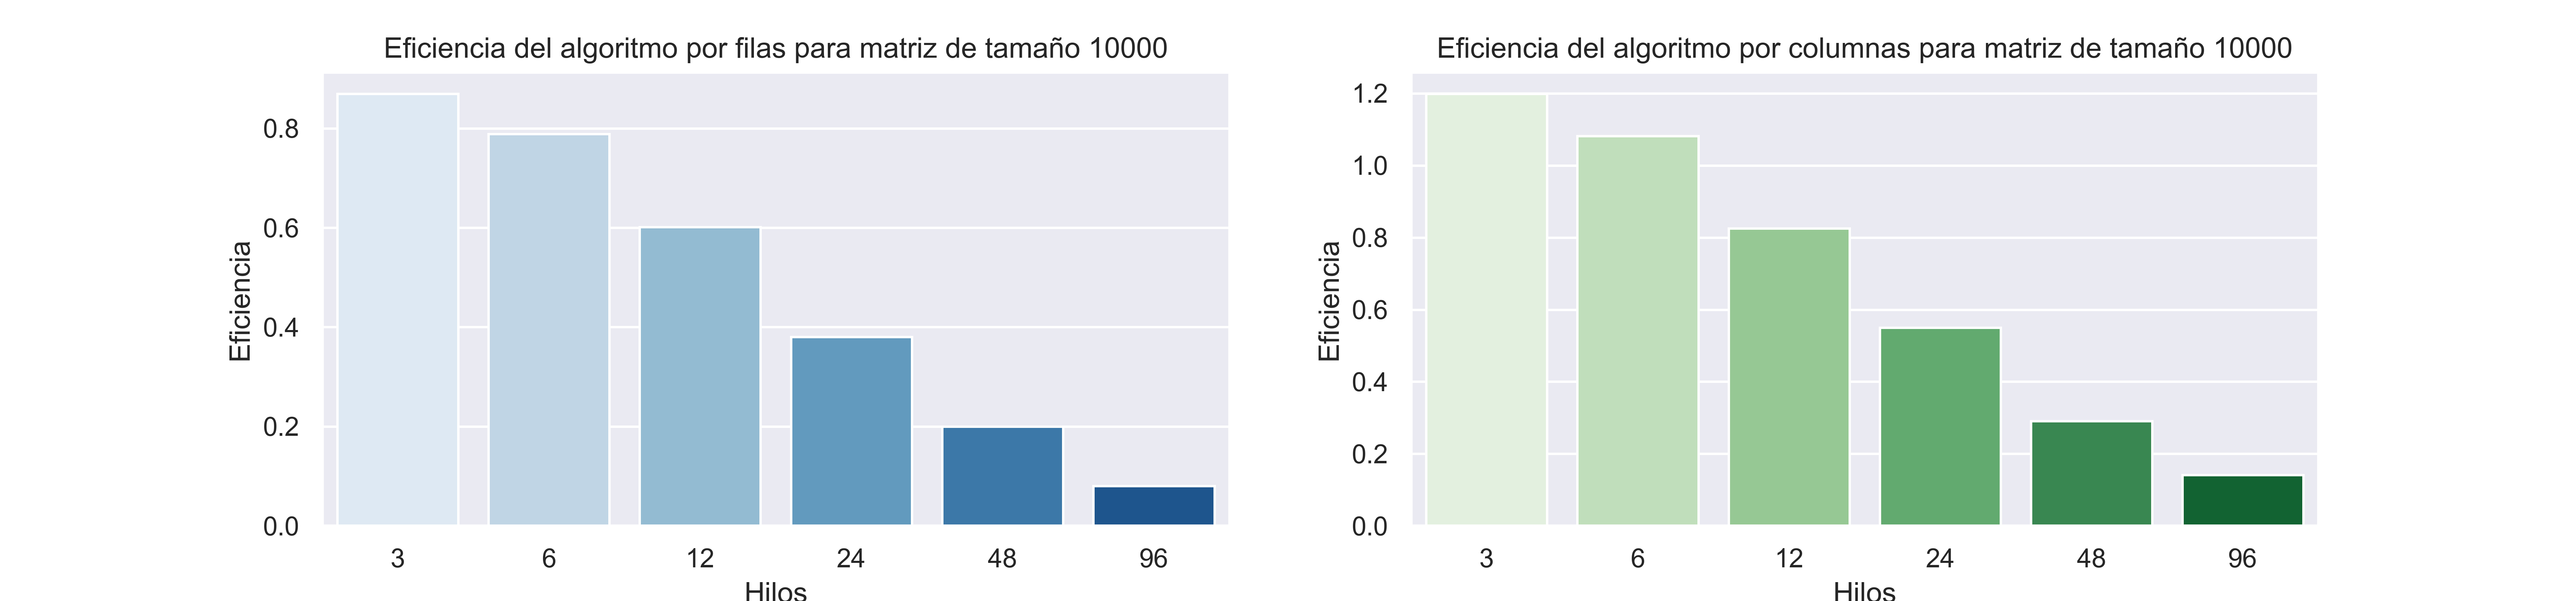
\includegraphics[width=\textwidth]{stars_eff_bar}
\label{fig:stareffbar}
\end{figure}

Para acabar, obervamos el overhead que sufren los algoritmos. Los resultados
son congruentes con la historia hasta ahora. El overhead aumenta con el número de
hilos, y ve un incremento dramatico en las corridas con 96 hilos. Estos resultados
estan graficados en la figura \ref{fig:staroverhead}

\begin{figure}[H]
    \centering
  \caption{Overhead de los algoritmos}
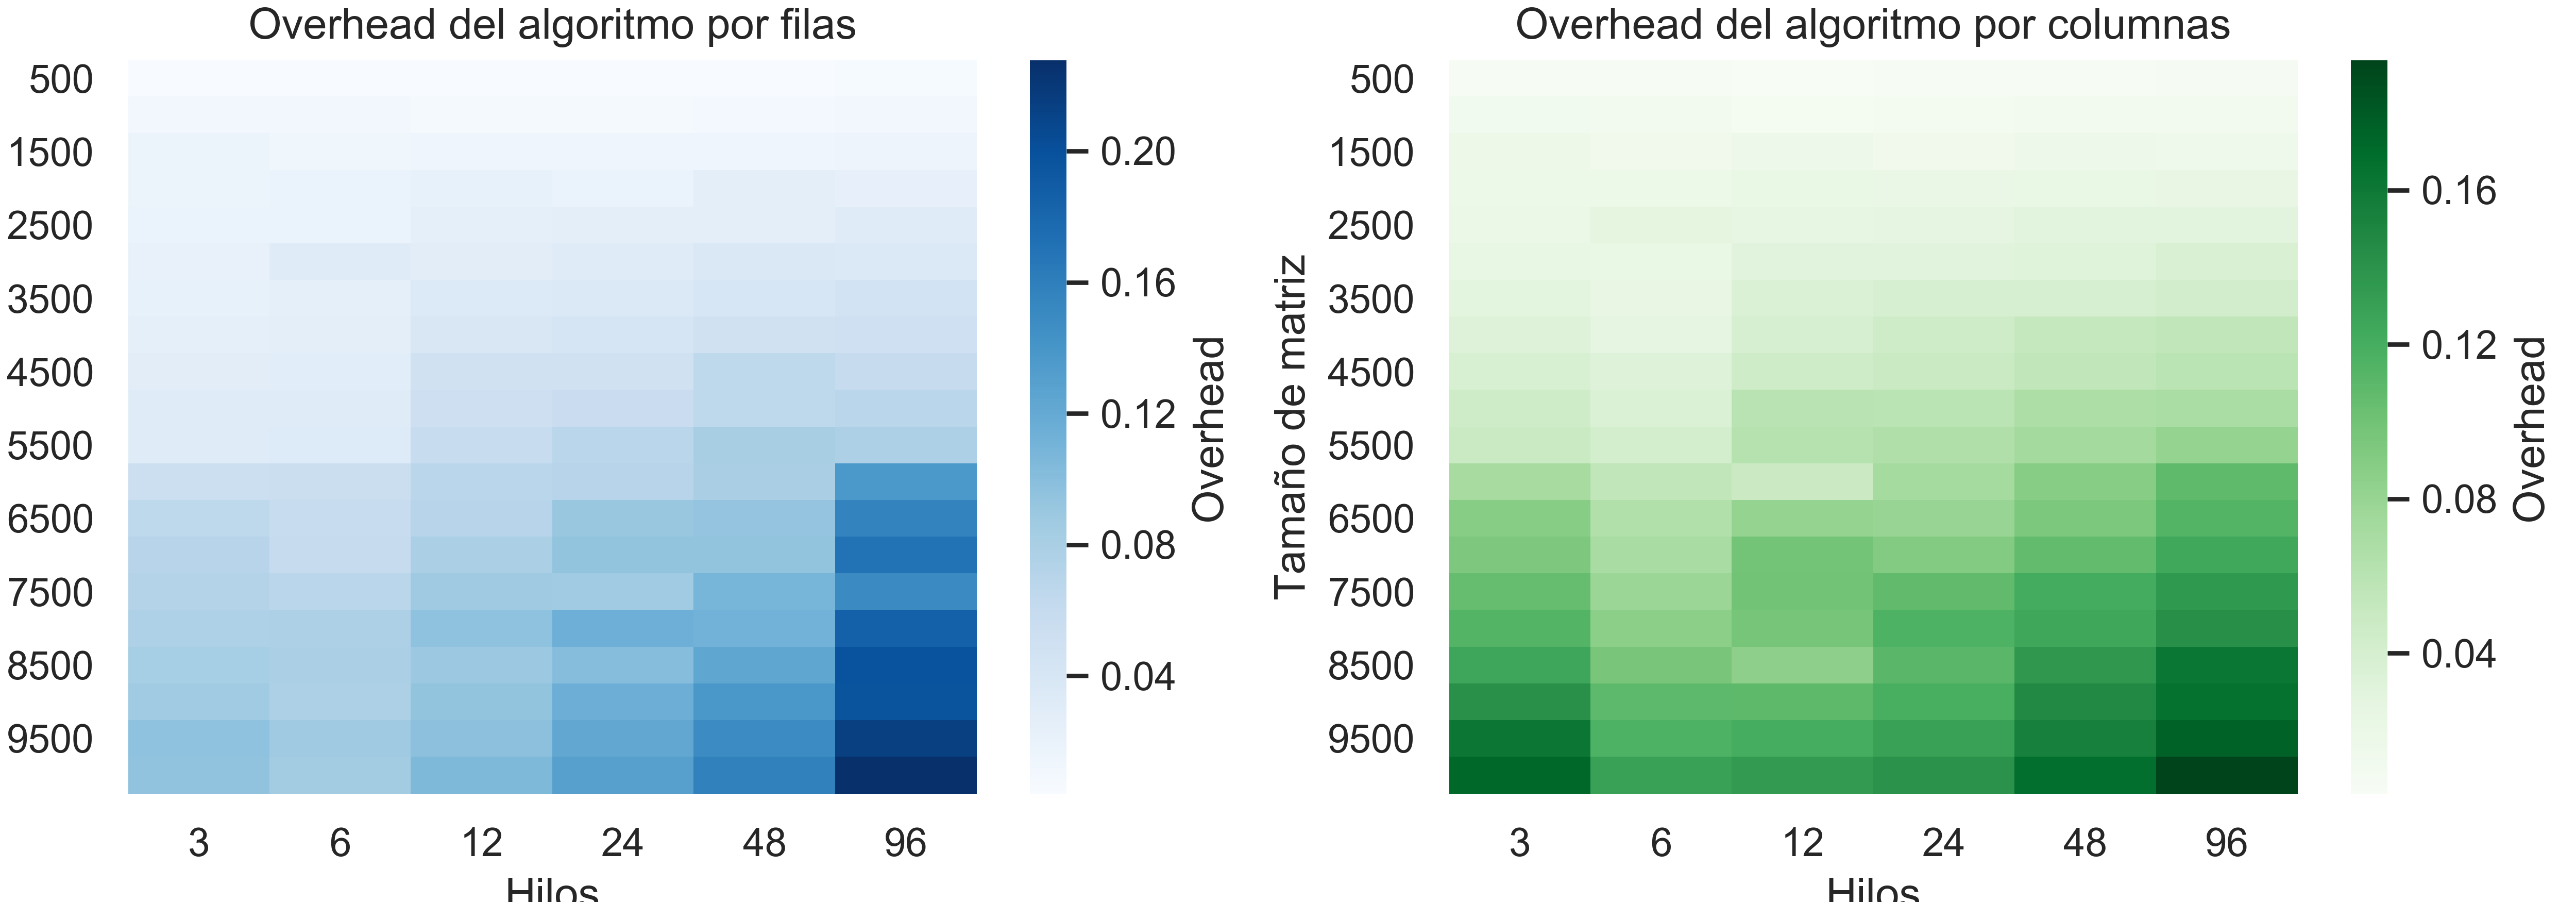
\includegraphics[width=\textwidth]{stars_overhead}
\label{fig:staroverhead}
\end{figure}

\section{Conclusión}

Ambos algoritmos de detección de estrellas nos muestran propiedades típicas de los
algoritmos distribuidos. Vemos que el algoritmo paralelo en general es mucho más
rapido que el secuencial. Pero tambien vemos que la eficiencia de uso de recursos
baja rapidamente entre mas paralelizemos el algoritmo.

Vemos tambien que hay cierto punto cuando agregar mas hilos se vuelve
contraproducente cuando la cantidad de hilos supere el numero de núcleos de
procesador con los que contamos. Este punto obviamente depende del procesador, pero
es importante estar consciente de su existencia.

\chapter{Problema 2}

\textbf{Enunciado} Analizar el desempeño del programa que calcula las raices
cuadradas entre $1$ y $n$.

\section{Descripción del algoritmo}

Los tres algoritmos son los vistos en clase:

\begin{itemize}
  \item El algoritmo secuencial original.
  \item El algoritmo paralelo usando un arreglo compartido, de aqui en adelante
    algoritmo 1.
  \item El algoritmo paralelo donde cada hilo regresa parte de la solución y el
    hilo principal las reune, de aqui en adelante algoritmo 2
\end{itemize}

\section{Experimentos}

Todos los experimentos se realizaron dentro del mismo entorno que el problema 1,
descritos en la tabla~\ref{table:testspecs}.

De nuevo, los expermientos paralelos se realizaron con 3, 6, 12, 24, 48 y 96 hilos.
En este caso se prob\'o el algoritmo para problemas de tamaño $N = 5000000x$ para
$x = 1, 2, \ldots, 19, 20$.

Se toma en cuenta la mediana de 50 ejecuciónes para reducir el impacto de factores
externos.

Comenzamos observando los tiempos de ejecución. La figura~\ref{fig:squareperf} nos
muestra la ejecución secuencial contra las ejecuciones en paralelo con 12 hilos.
Vemos que en general ambas versiones paralelas nos ofrecen una gran mejora frente
a la secuencial.

En la derecha vemos una comparación solo entre las dos versiones paralelas. Vemos
que la version que comparte memoria entre hilos es ligeramente más lenta que la
version donde cada hilo regresa reultados parciales.

\begin{figure}[H]
    \centering
  \caption{Desempeño de los algoritmos}
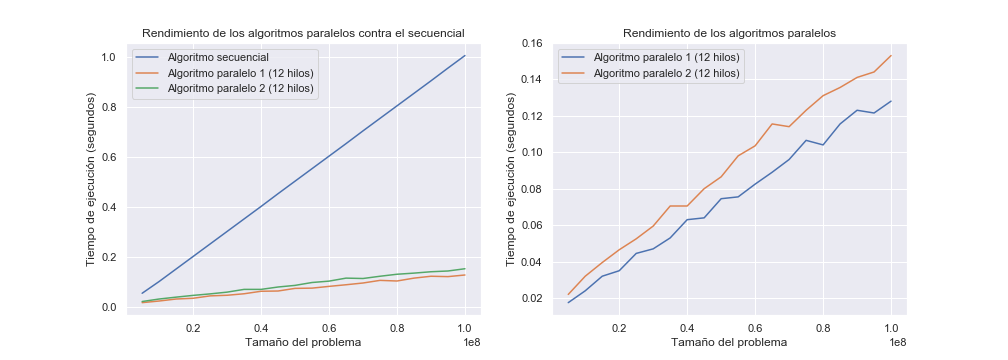
\includegraphics[width=\textwidth]{square-perf}
\label{fig:squareperf}
\end{figure}

Nos tornamos a un ejemplo de tamaño $100,000,000$ para analizar el cambio en el
desempeño mientras varía el numero de hilos. En la figura~\ref{fig:squareperfbar}
vemos como el desempeño en realidad se reduce cuando aumentamos el numero de hilos
sobre cierto punto, sugiriendo que el tamaño del problema no es lo suficientemente
grande para que el berneficio de la paralelización supere el costo del overhead de
dividir el trabajo.

\begin{figure}[H]
    \centering
  \caption{Desempeño de los algoritmos}
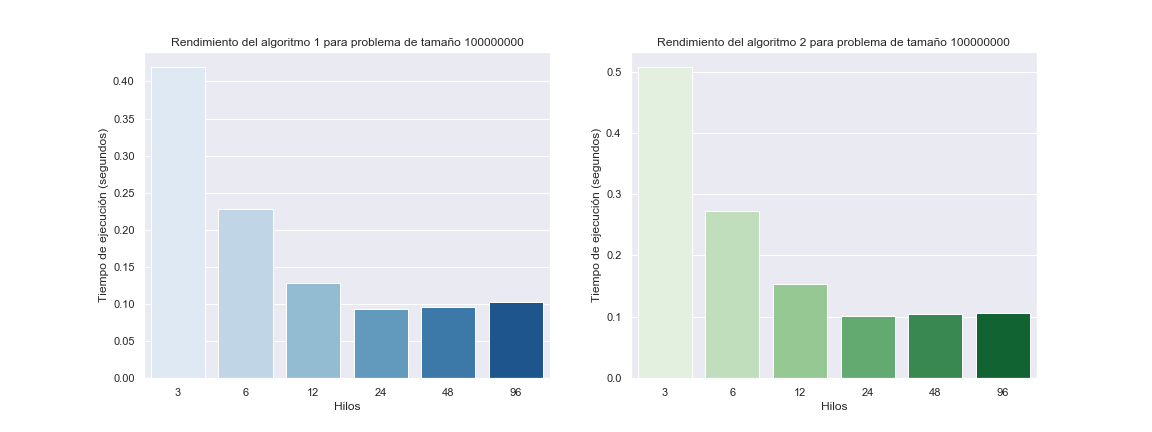
\includegraphics[width=\textwidth]{square-perf-bar}
\label{fig:squareperfbar}
\end{figure}

Nos tornamos ahora a la aceleración, ilustrada en la figura~\ref{fig:squareaccel}.
Vemos un resultado que corrobora el punto pasado. La aceleración aumenta rapidamente
hasta llegar a 24 hilos, de ahi comienza a decrecer. Este comportamiento se puede
ver mas claro en el caso especifico de $N = 100,000,000$, graficado en la figura
\ref{fig:squareaccelbar}. Tambien vemos de nuevo que el algoritmo 2 tiene una
ligera ventaja sobre el algoritmo 1.

\begin{figure}[H]
    \centering
  \caption{Aceleración de los algoritmos}
  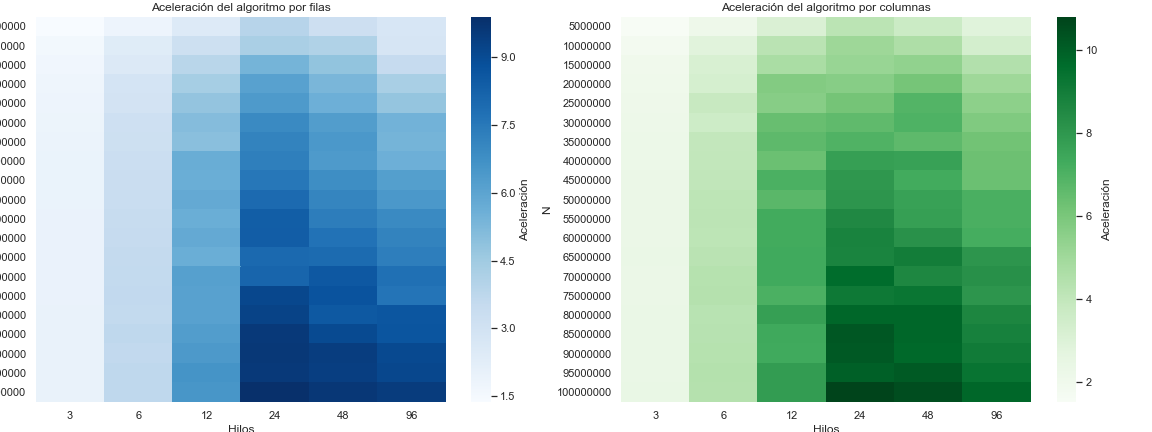
\includegraphics[width=\textwidth]{square-accel}
\label{fig:squareaccel}
\end{figure}

\begin{figure}[H]
    \centering
  \caption{Aceleración de los algoritmos}
  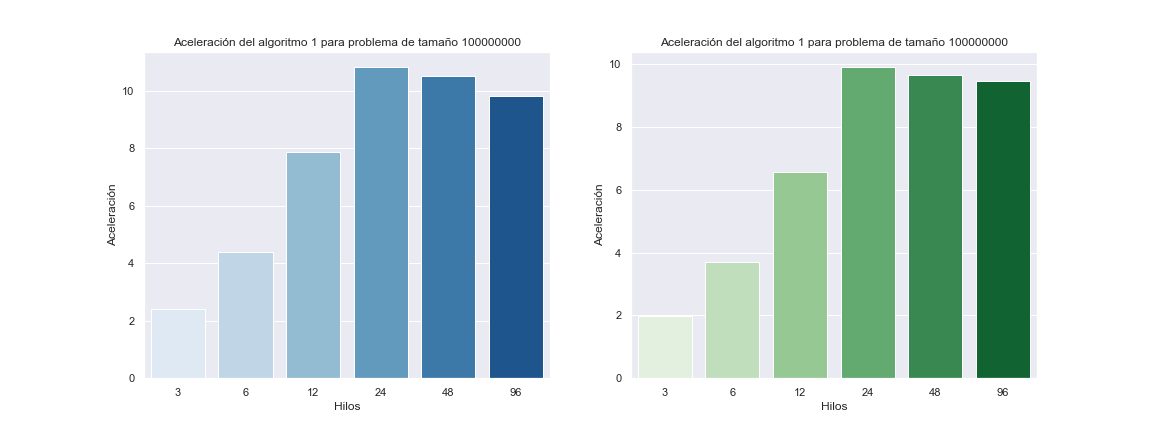
\includegraphics[width=\textwidth]{square-accel-bar}
\label{fig:squareaccelbar}
\end{figure}

El siguiente punto a analizar es la eficiencia de ambos algoritmos frente a sus
versiones secuenciales. Un mapa de calor de estos datos se encuentra en la figura
\ref{fig:squareeff}. Al igual que en el problema anterior se observa que la
baja mientras el número de hilos aumenta y sube junto con el tamaño del problema.
En la figura\ref{fig:squareeffbar}, especifica para $N = 100,000,000$, podemos
observar una repentina reducción en eficiencia al pasar de 24 a 48 hilos,
continuando la historia que contaban los resultados anteriores.

\begin{figure}[H]
    \centering
  \caption{Eficiencia de los algoritmos}
  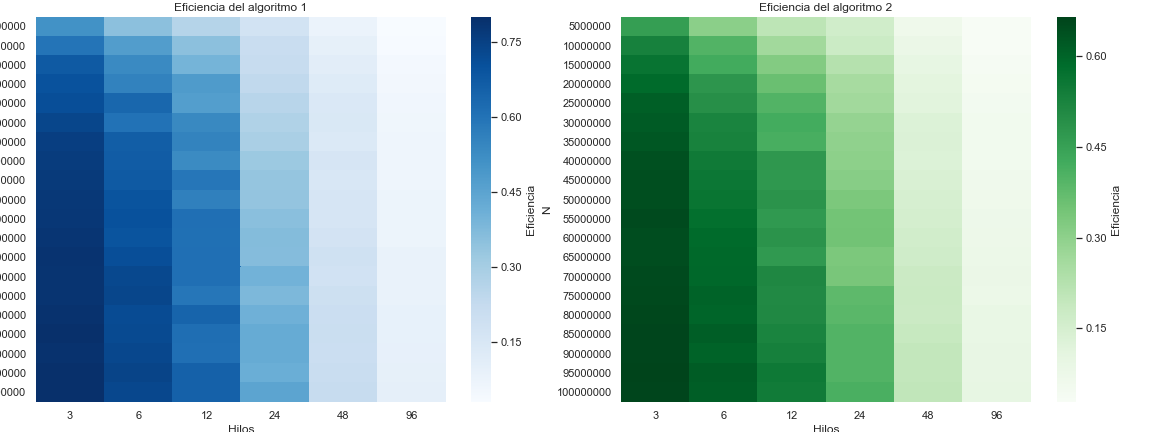
\includegraphics[width=\textwidth]{square-eff}
\label{fig:squareeff}
\end{figure}

\begin{figure}[H]
    \centering
  \caption{Eficiencia de los algoritmos}
  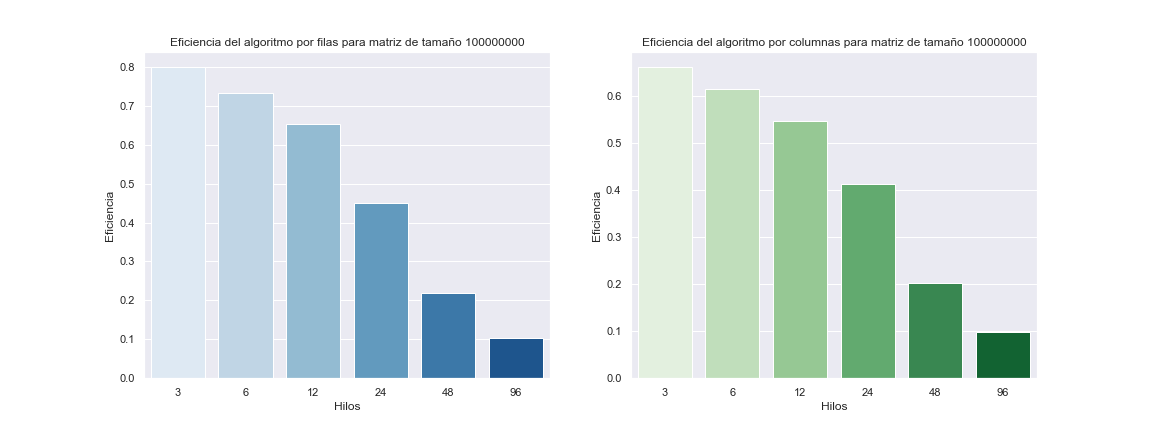
\includegraphics[width=\textwidth]{square-eff-bar}
\label{fig:squareeffbar}
\end{figure}

Finalemente observaremos la figura \ref{fig:squareoverhead}, donde se muestran los
valores de overhead. Curiosamente vemos que a diferencia del problema anterior, donde
el overhead se reducia entre menos hilos crearamos, acá vemos que el punto minimo de
overhead es entre 12 y 24 hilos. Vemos tambien que el overhead se maximiza despues de
24 hilos, el punto donde el algoritmo deja de acelerar entre mas hilos arrojemos al
problema.

\begin{figure}[H]
    \centering
  \caption{Overhead de los algoritmos}
  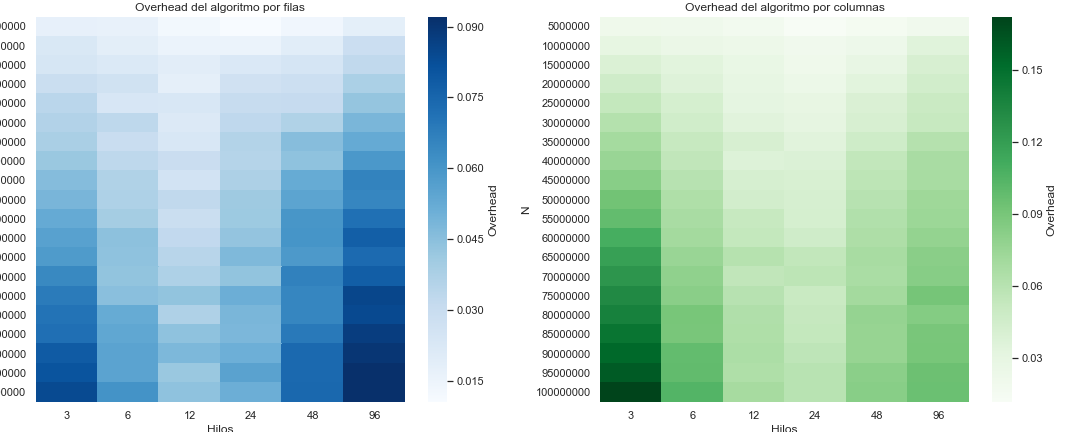
\includegraphics[width=\textwidth]{square-overhead}
\label{fig:squareoverhead}
\end{figure}

\section{Conclusión}

En este ejercicio se puede observar que el punto donde agregar mas hilos deja de ser
beneficioso no necesariamente depende del numero de hilos que se pueden ejecutar
concurrentemente. El factor mas importante en realidad es la relación entre el
beneficio de dividir el problema y el costo de crear estas divisiones y reunir los
resultados. En este caso rapidamente nos topamos con el punto donde el overhead
de paralelizar de más terminó alentando el desempeño de la solución.

\chapter{Problema 3}

Construir un programa paralelo que tome como entrada un conjunto de n elementos
almacenados en una lista y generar su conjunto potencia.

\section{Algoritmo}

Para la versión secuencial utilizamos este algoritmo. Usamos la representación
de bits para generar los conjuntos fuera de orden, luego usamos un ordenamiento
por conteo para arreglar el orden.

\begin{algorithm}
\caption{Conjinto potencia secuencial}\label{euclid}
\begin{algorithmic}[1]
\Procedure{Potencia}{$N$}\Comment{Conjunto potencia secuencial}
\State Inicializar $S$ con $2^N$ conjuntos vacios
\For{$i$ in $1..2^N$}
  \For{$j$ in $1..N$}
    \If{El bit $j$ está encendido en el numero $i$}
      \State Agregar el elemento $j$ de la lista de entrada al conjunto $i$
    \EndIf
  \EndFor
\EndFor
\State CountingSort($S$)
\EndProcedure
\end{algorithmic}
\end{algorithm}

Para la versión paralela, dividimos la sección de generar los conjuntos desordenados
en hilos, y luego tambien usamos una version paralela del counting sort para
intentar acelerar ese paso.

\subsection{Analisís de complejidad}

El algoritmo tiene complejidad $O(n2^n)$.

\section{Expermientos}

Los experimentos se llevaron a cabo en el mismo servidor que los problemas
anteriores, especificado en la tabla \ref{table:testspecs}.

Se probó de nuevo para $3, 6, 12, 24, 48, 96$ hilos, con tamaños de problema
$n = 15, 16, \ldots, 24, 25$. Se repitió el experimento 5 veces, tomando en cuenta
el valor mediano. Los resultados se encuentran en el apendice C.

Resulta que paralelizar este algoritmo en particular tuvo un efecto terrible.
Observemos la figura \ref{fig:powersetperf}. El algoritmo en todos los casos
corre mas lento en su versión paralela. El rendimiento se vuelve peor entre más
hilos se agreguén. No estoy seguro de que ocasiona que se alente.

\begin{figure}[H]
    \centering
    \caption{Rendimiento del algoritmo}
  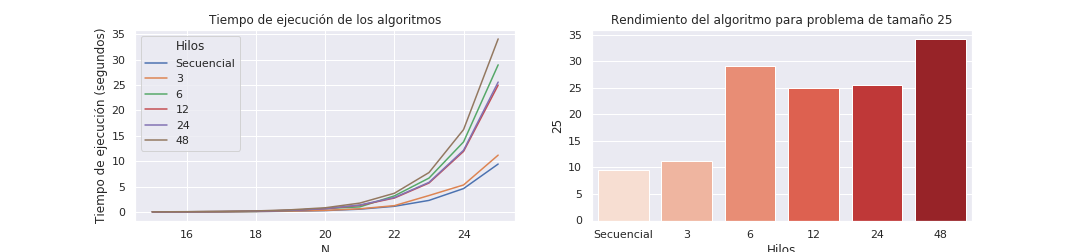
\includegraphics[width=\textwidth]{powerset-perf}
\label{fig:powersetperf}
\end{figure}

La aceleración muestra lo mismo. El algoritmo paralelo en ningun punto es más
rapido. Tal véz esto diga mas sobre la rápidez del algoritmo secuencial que nada.

\begin{figure}[H]
    \centering
    \caption{Aceleración del algoritmo}
  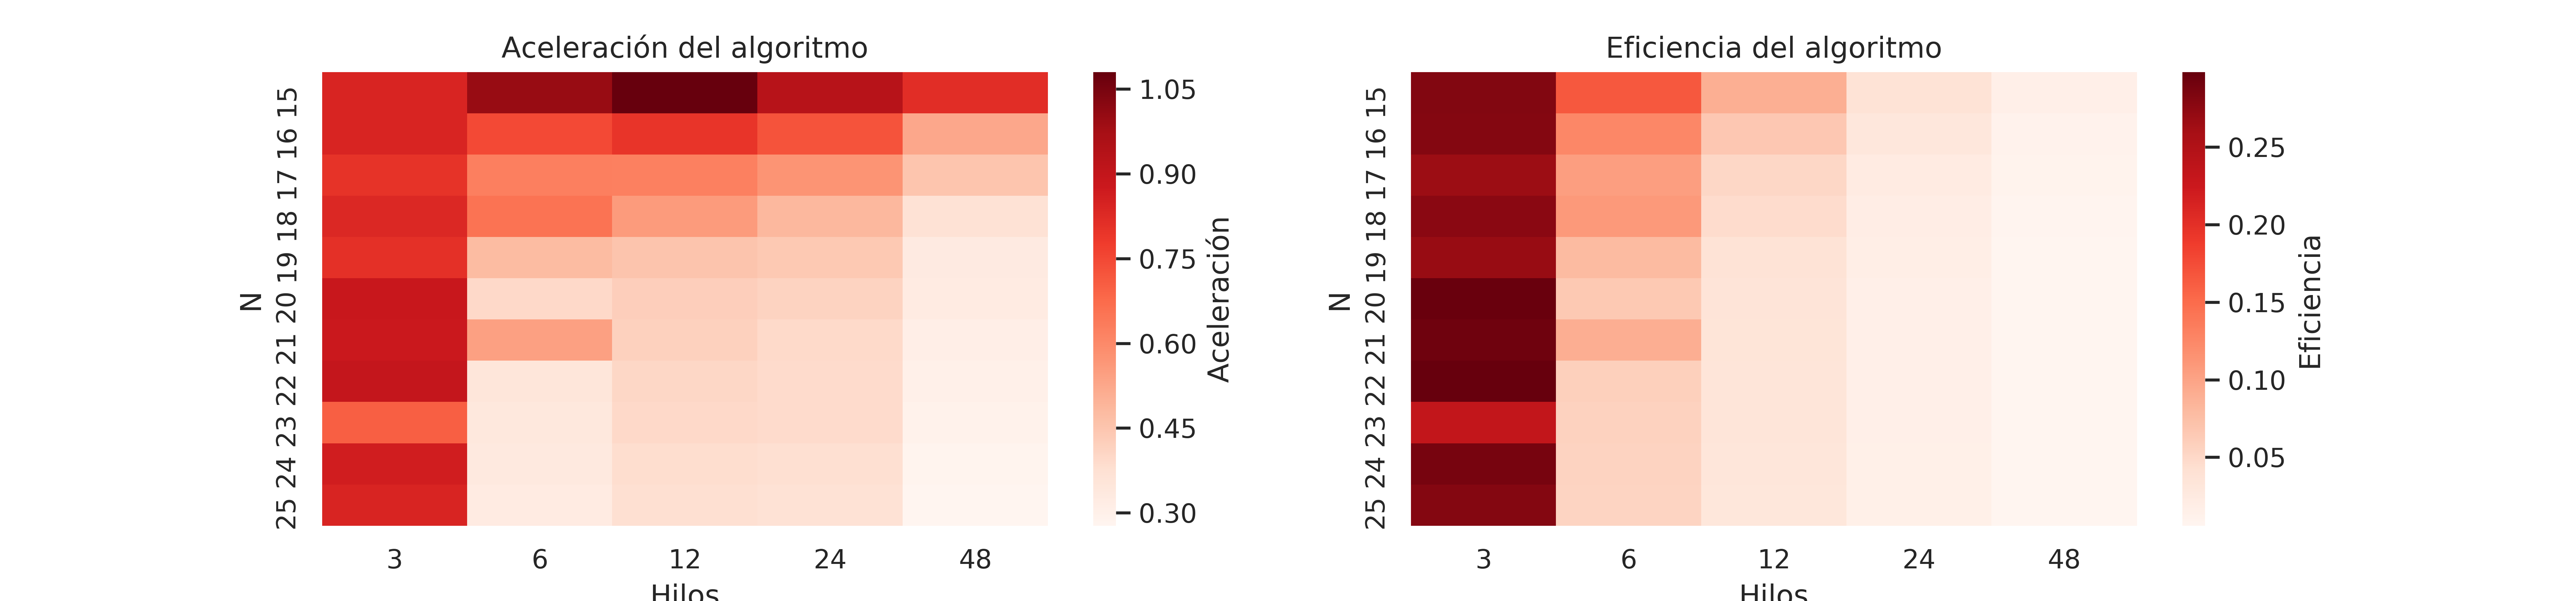
\includegraphics[width=\textwidth]{powerset-accel}
\label{fig:powersetaccel}
\end{figure}

\section{Conclusión}

Este problema remarca la dificultad de diseñar algoritmos paralelos.
Se ve que el costo de crear hilos a menudo dificulta diseñar estos algoritmos.
Hay distintos enfoques para diseñar estos algoritmos pero hay algunos que llevan
a mas exito que otros. Hay que buscar el enfoque correcto y en este caso no
se encontró.

%
\begin{appendices}

\chapter{Datos experimentales del problema 1}
\label{appendix:starresults}

\begin{table}[H]
\begin{tabular}{lrrrrrrr}
\toprule
Hilos &  Secuencial &       3 &       6 &      12 &      24 &      48 &      96 \\
Tamaño de matriz &             &         &         &         &         &         &         \\
\midrule
500              &      0.0050 &  0.0060 &  0.0050 &  0.0050 &  0.0050 &  0.0050 &  0.0060 \\
1000             &      0.0190 &  0.0180 &  0.0135 &  0.0100 &  0.0090 &  0.0100 &  0.0110 \\
1500             &      0.0420 &  0.0310 &  0.0200 &  0.0190 &  0.0160 &  0.0150 &  0.0160 \\
2000             &      0.0750 &  0.0420 &  0.0315 &  0.0280 &  0.0230 &  0.0290 &  0.0235 \\
2500             &      0.1170 &  0.0580 &  0.0390 &  0.0345 &  0.0315 &  0.0295 &  0.0320 \\
3000             &      0.1680 &  0.0770 &  0.0590 &  0.0420 &  0.0380 &  0.0400 &  0.0380 \\
3500             &      0.2300 &  0.0990 &  0.0630 &  0.0540 &  0.0460 &  0.0455 &  0.0485 \\
4000             &      0.3000 &  0.1250 &  0.0775 &  0.0640 &  0.0550 &  0.0550 &  0.0540 \\
4500             &      0.3800 &  0.1545 &  0.0920 &  0.0805 &  0.0650 &  0.0740 &  0.0640 \\
5000             &      0.4680 &  0.1870 &  0.1090 &  0.0915 &  0.0755 &  0.0755 &  0.0730 \\
5500             &      0.5740 &  0.2225 &  0.1295 &  0.1055 &  0.0925 &  0.0935 &  0.0840 \\
6000             &      0.6820 &  0.2810 &  0.1690 &  0.1250 &  0.0995 &  0.0935 &  0.1445 \\
6500             &      0.8000 &  0.3325 &  0.1910 &  0.1380 &  0.1240 &  0.1100 &  0.1650 \\
7000             &      0.9250 &  0.3790 &  0.2140 &  0.1560 &  0.1330 &  0.1135 &  0.1805 \\
7500             &      1.0680 &  0.4290 &  0.2460 &  0.1765 &  0.1310 &  0.1320 &  0.1605 \\
8000             &      1.2200 &  0.4840 &  0.2815 &  0.1980 &  0.1655 &  0.1375 &  0.1980 \\
8500             &      1.3680 &  0.5385 &  0.3070 &  0.2030 &  0.1580 &  0.1525 &  0.2125 \\
9000             &      1.5315 &  0.5970 &  0.3330 &  0.2220 &  0.1790 &  0.1705 &  0.2130 \\
9500             &      1.7110 &  0.6670 &  0.3725 &  0.2410 &  0.1940 &  0.1845 &  0.2320 \\
10000            &      1.9020 &  0.7290 &  0.4020 &  0.2635 &  0.2085 &  0.1980 &  0.2475 \\
\bottomrule
\end{tabular}
\caption{Valor mediano del tiempo de ejecución del algoritmo por filas
  considerando 40 ejecuciones}
\label{table:squares-alg1-data}
\end{table}

\begin{table}[H]

  \begin{tabular}{lrrrrrrr}
\toprule
Hilos &  Secuencial &       3 &       6 &      12 &      24 &      48 &      96 \\
Tamaño de matriz &             &         &         &         &         &         &         \\
\midrule
500              &      0.0050 &  0.0065 &  0.0055 &  0.0040 &  0.0050 &  0.0050 &  0.0060 \\
1000             &      0.0200 &  0.0180 &  0.0135 &  0.0100 &  0.0100 &  0.0100 &  0.0110 \\
1500             &      0.0420 &  0.0310 &  0.0205 &  0.0200 &  0.0150 &  0.0170 &  0.0155 \\
2000             &      0.0780 &  0.0430 &  0.0305 &  0.0290 &  0.0240 &  0.0230 &  0.0250 \\
2500             &      0.1230 &  0.0595 &  0.0470 &  0.0355 &  0.0310 &  0.0325 &  0.0305 \\
3000             &      0.1800 &  0.0790 &  0.0500 &  0.0450 &  0.0380 &  0.0360 &  0.0390 \\
3500             &      0.2510 &  0.1050 &  0.0620 &  0.0550 &  0.0490 &  0.0440 &  0.0455 \\
4000             &      0.3430 &  0.1340 &  0.0770 &  0.0645 &  0.0580 &  0.0585 &  0.0580 \\
4500             &      0.4480 &  0.1650 &  0.0960 &  0.0780 &  0.0650 &  0.0640 &  0.0625 \\
5000             &      0.5780 &  0.2025 &  0.1140 &  0.0985 &  0.0785 &  0.0775 &  0.0740 \\
5500             &      0.7185 &  0.2405 &  0.1375 &  0.1095 &  0.0895 &  0.0850 &  0.0875 \\
6000             &      0.9020 &  0.2990 &  0.1690 &  0.1050 &  0.1010 &  0.1025 &  0.1150 \\
6500             &      1.0575 &  0.3550 &  0.1980 &  0.1480 &  0.1130 &  0.1110 &  0.1225 \\
7000             &      1.2730 &  0.4020 &  0.2250 &  0.1760 &  0.1295 &  0.1260 &  0.1340 \\
7500             &      1.5030 &  0.4610 &  0.2560 &  0.1890 &  0.1515 &  0.1435 &  0.1465 \\
8000             &      1.7465 &  0.5205 &  0.2900 &  0.1990 &  0.1670 &  0.1505 &  0.1555 \\
8500             &      1.9695 &  0.5820 &  0.3240 &  0.1990 &  0.1680 &  0.1655 &  0.1765 \\
9000             &      2.2920 &  0.6525 &  0.3650 &  0.2360 &  0.1825 &  0.1795 &  0.1815 \\
9500             &      2.5850 &  0.7315 &  0.4010 &  0.2630 &  0.2005 &  0.1900 &  0.1940 \\
10000            &      2.8975 &  0.8055 &  0.4465 &  0.2925 &  0.2195 &  0.2075 &  0.2135 \\
\bottomrule
\end{tabular}

\caption{Valor mediano del tiempo de ejecución del algoritmo por columnas
  considerando 40 ejecuciones}
\label{table:squares-alg1-data}
\end{table}

\chapter{Datos experimentales del problema 2}

\begin{table}[H]
\begin{tabular}{lrrrrrrr}
\toprule
Hilos &  Secuencial &       3 &       6 &      12 &      24 &      48 &      96 \\
N         &             &         &         &         &         &         &         \\
\midrule
5000000   &       0.055 &  0.0360 &  0.0260 &  0.0175 &  0.0130 &  0.0150 &  0.0190 \\
10000000  &       0.102 &  0.0570 &  0.0360 &  0.0240 &  0.0200 &  0.0220 &  0.0300 \\
15000000  &       0.152 &  0.0750 &  0.0475 &  0.0320 &  0.0290 &  0.0280 &  0.0340 \\
20000000  &       0.202 &  0.0965 &  0.0605 &  0.0350 &  0.0355 &  0.0330 &  0.0400 \\
25000000  &       0.252 &  0.1180 &  0.0660 &  0.0445 &  0.0410 &  0.0365 &  0.0455 \\
30000000  &       0.302 &  0.1370 &  0.0835 &  0.0470 &  0.0455 &  0.0430 &  0.0515 \\
35000000  &       0.352 &  0.1555 &  0.0885 &  0.0530 &  0.0505 &  0.0530 &  0.0565 \\
40000000  &       0.402 &  0.1760 &  0.1000 &  0.0630 &  0.0520 &  0.0525 &  0.0635 \\
45000000  &       0.453 &  0.1970 &  0.1120 &  0.0640 &  0.0565 &  0.0620 &  0.0710 \\
50000000  &       0.503 &  0.2165 &  0.1210 &  0.0745 &  0.0620 &  0.0655 &  0.0705 \\
55000000  &       0.553 &  0.2370 &  0.1315 &  0.0755 &  0.0645 &  0.0715 &  0.0775 \\
60000000  &       0.603 &  0.2570 &  0.1450 &  0.0825 &  0.0685 &  0.0730 &  0.0835 \\
65000000  &       0.653 &  0.2760 &  0.1530 &  0.0890 &  0.0745 &  0.0725 &  0.0805 \\
70000000  &       0.704 &  0.2990 &  0.1610 &  0.0960 &  0.0730 &  0.0815 &  0.0850 \\
75000000  &       0.754 &  0.3200 &  0.1710 &  0.1065 &  0.0825 &  0.0810 &  0.0930 \\
80000000  &       0.804 &  0.3390 &  0.1865 &  0.1040 &  0.0820 &  0.0820 &  0.0925 \\
85000000  &       0.854 &  0.3570 &  0.1965 &  0.1155 &  0.0835 &  0.0870 &  0.0965 \\
90000000  &       0.904 &  0.3800 &  0.2060 &  0.1230 &  0.0885 &  0.0930 &  0.0995 \\
95000000  &       0.955 &  0.3990 &  0.2145 &  0.1215 &  0.0955 &  0.0940 &  0.1020 \\
100000000 &       1.005 &  0.4190 &  0.2285 &  0.1280 &  0.0930 &  0.0955 &  0.1025 \\
\bottomrule
\end{tabular}
\caption{Valor mediano del tiempo de ejecución del algoritmo 1
  considerando 40 ejecuciones}
\label{table:squares-alg1-data}
\end{table}

\begin{table}[H]
\begin{tabular}{lrrrrrrr}
\toprule
Hilos &  Secuencial &       3 &       6 &      12 &      24 &      48 &      96 \\
N         &             &         &         &         &         &         &         \\
\midrule
5000000   &       0.055 &  0.0400 &  0.0300 &  0.0220 &  0.0140 &  0.0170 &  0.0200 \\
10000000  &       0.102 &  0.0640 &  0.0425 &  0.0320 &  0.0240 &  0.0250 &  0.0360 \\
15000000  &       0.152 &  0.0895 &  0.0595 &  0.0395 &  0.0280 &  0.0315 &  0.0430 \\
20000000  &       0.202 &  0.1140 &  0.0700 &  0.0465 &  0.0330 &  0.0380 &  0.0470 \\
25000000  &       0.252 &  0.1375 &  0.0850 &  0.0525 &  0.0395 &  0.0450 &  0.0530 \\
30000000  &       0.302 &  0.1625 &  0.0960 &  0.0595 &  0.0435 &  0.0480 &  0.0550 \\
35000000  &       0.352 &  0.1870 &  0.1105 &  0.0705 &  0.0490 &  0.0545 &  0.0650 \\
40000000  &       0.402 &  0.2090 &  0.1220 &  0.0705 &  0.0550 &  0.0630 &  0.0720 \\
45000000  &       0.453 &  0.2340 &  0.1355 &  0.0800 &  0.0600 &  0.0665 &  0.0730 \\
50000000  &       0.503 &  0.2605 &  0.1485 &  0.0865 &  0.0630 &  0.0705 &  0.0780 \\
55000000  &       0.553 &  0.2830 &  0.1600 &  0.0980 &  0.0660 &  0.0750 &  0.0795 \\
60000000  &       0.603 &  0.3105 &  0.1705 &  0.1035 &  0.0715 &  0.0780 &  0.0840 \\
65000000  &       0.653 &  0.3360 &  0.1840 &  0.1155 &  0.0815 &  0.0820 &  0.0890 \\
70000000  &       0.704 &  0.3600 &  0.1970 &  0.1140 &  0.0865 &  0.0820 &  0.0905 \\
75000000  &       0.754 &  0.3840 &  0.2080 &  0.1230 &  0.0825 &  0.0860 &  0.0985 \\
80000000  &       0.804 &  0.4065 &  0.2240 &  0.1310 &  0.0865 &  0.0940 &  0.0930 \\
85000000  &       0.854 &  0.4310 &  0.2320 &  0.1355 &  0.0890 &  0.0945 &  0.0985 \\
90000000  &       0.904 &  0.4550 &  0.2490 &  0.1410 &  0.0940 &  0.0955 &  0.0995 \\
95000000  &       0.955 &  0.4785 &  0.2580 &  0.1440 &  0.0995 &  0.1015 &  0.1045 \\
100000000 &       1.005 &  0.5070 &  0.2725 &  0.1530 &  0.1015 &  0.1040 &  0.1060 \\
\bottomrule
\end{tabular}
\caption{Valor mediano del tiempo de ejecución del algoritmo 2
  considerando 40 ejecuciones}
\label{table:squares-alg2-data}
\end{table}
\end{appendices}


\end{document}
